\chapter{Data Model}
\section{Document Database - MongoDB}
Starting to reason from the queries we wanted to run against our database, we started the modeling process deciding to use a Document Database, that allows for scalability and flexibility. It did seem like the most reasonable choice by looking at the amount of data we needed to deal with.
\subsection{Document DB Collections}
\subsubsection{Videogames}
Whenever a videogame document is inserted, company managers may choose any number of attributes to add to it, of any significance. However, we defined the following attributes to be mandatory when a new videogame is created:
\begin{itemize}
	\item \texttt{Name}
        \item \texttt{Description}
        \item \texttt{Image}
	\item \texttt{Release Date}
	\item \texttt{Platform} 
	\item \texttt{Publishers} 
	\item \texttt{Developers}
        \item \texttt{Genre}
\end{itemize}
Of those, \emph{Name}, \emph{Release Date}, \emph{Publishers} and \emph{Developers} are the attributes that are the focus of the analytic queries that we run.
A videogame also has the following attributes:
\begin{itemize}
    \item \texttt{reviews}: here we find all the reviews related to a specific videogame, in a simplified form; the attributes stored are "reviewId, score, author, date". 
    \item \texttt{user\_review}: it holds the average score for the game.  
    \item \texttt{reviewCount}: it holds the total count of reviews for the game.
    \item \texttt{Top3ReviewsByLikes}: it embeds the top 3 reviews (with all their attributes) for the game by amount of likes received.
\end{itemize}
The first three are updated every time a review is added or deleted from the database. Updating the last one is an expensive operation, so it is done only periodically, or whenever an administrator requests it.
\subsubsection{Users}
As previously said a \emph{user} can either be a simple \emph{reviewer}, a \emph{Company Manager} or an \emph{Administrator} (look below at attributes \texttt{company\_name} ans \texttt{is\_admin} to see how to discriminate between the various types of users). 
Here we have some of the attributes we may find in a typical user's document :
\begin{itemize}
    \item \texttt{username} : it is a unique string that identifies a specific user into the database. It is set during the \emph{sign up} procedure after checking the chosen username is not associated to an already existing account.
    \item \texttt{email} : string that contains the email given during the \emph{sign up} procedure.
    \item \texttt{password\_hash} : string that contains the hash of the password chosen during the \emph{sign up} procedure .
    %\item \texttt{image} : string containing the URL of an image that may or may not be given at the time of the \emph{sign up} procedure. If not, a default image will be assigned to said user.
    \item \texttt{company\_name} : string that if present into a user's document identifies that user as a \emph{Company Manager}.
    \item \texttt{is\_admin} : boolean value, if set to \emph{true} in a user's document than that user is identified as an \emph{Administrator}.
\end{itemize}
\subsubsection{Companies}
\begin{itemize}
    \item \texttt{Name} : string that uniquely identifies a Company. It is mandatory to have a name associated to each Company in the system. 
    \item \texttt{imglink} : string that may or may not be present, containing the URL of an image linked to the specific Company it is attached to.
    \item \texttt{Overview} : string that may or may not be present. It contains informations about the Company.
    \item \texttt{Top3Games} : here we have the top three videogames owned by the Company embedded. The average score of each videogame may of course change over time, so we periodically update the three embedded documents (if needed). Being a quite expensive operation, the update gets scheduled periodically - or whenever the administrator requests it. 
\end{itemize}
\subsubsection{Reviews}
We did consider the possibility to embed entirely the reviews (i.e. including their actual content, the text - here into the \texttt{quote} attribute) into the videogames collection (or even the users one), but we soon realized the amount of expected data, all together, could grow too much, making the aggregations we perform over reviews heavier and much slower. Moreover we'd have a maximum number of storable reviews that would get around $25k$ reviews per videogame (or user). We settled for a reduced version (not including content) of each review embedded into the specific document representing the videogame it was written for. This way we have a list for every videogame of its reviews, which is accessible directly from the videogames' collection, plus the review collection that contains all the reviews' details.
\begin{itemize}
    \item \texttt{score} : each review has to have a score attached to it.
    \item \texttt{quote} : text of the review.
    \item \texttt{author} : each review belongs to a specific user, here we find the related \texttt{username}.
    \item \texttt{date} : date of creation of the review in format \texttt{yyyy-MM-dd}.
    \item \texttt{likes} : integer that holds the number of likes of each specific review, updated at every added or deleted like.
\end{itemize}
\subsubsection{Comments}
\begin{itemize}
    \item \texttt{reviewId}: id of the review the comment is for.
    \item \texttt{author} : each comment belongs to a specific user, here we find the related \texttt{username}. 
    \item \texttt{quote} : text of the comment.
    \item \texttt{date} : date of creation of the comment in format \texttt{yyyy-MM-dd}.
\end{itemize}
As in the previous case we considered the possibility to embed comments into the reviews collection, each comment as an element of an array containing all the comments related to a specific review, but just as before we realized the document size could grow quickly with the average amount of comments we expect to have for each review. Again, aggregations would get heavier and that is what makes embedding not a viable possibility, even more so if we consider we are dealing with a relatively \emph{small} social network and some of the heavier aggregations (especially the ones we need to perform relatively rarely), already as it is, take in the order of $10s$ to complete. 
\subsubsection{User Images}
\begin{itemize}
    \item \texttt{username}
    \item \texttt{image}
\end{itemize}
We decided to add this redundancy to improve the performance of all the operations that require to show users' images, having compared the performance results obtained with and without it.
%\subsection{Document DB Relationships}
\subsection{Document DB Examples}
\subsubsection{Videogame}
\begin{lstlisting}[language = Java , frame = trBL , firstnumber = 1, escapeinside={(*@}{@*)}]
{
  "_id": {
    "$oid": "000000000000000000000001"
  },
  "Name": "(Almost) Total Mayhem",
  "Released": {
    "Release Date": "2011-01-14",
    "Platform": "Xbox 360"
  },
  "Publishers": "Peanut Gallery",
  "Developers": "Peanut Gallery",
  "Genre": "Action",
  "Perspective": "Side view",
  "Gameplay": "Platform",
  "Setting": "Fantasy",
  "Media Type": "Download",
  "Multiplayer Options": "Same/Split-Screen",
  "Number of Offline Players": "1-2 Players",
  "Description": "(Almost) Total Mayhem is a 2D team-based action platformer ...",
  "img": "https://cdn.mobygames.com/4b4ee410-ab7c-11ed-93d8-02420a000198.webp",
  "user_review": 6,
  "reviews": [
    {
      "reviewId": {
        "$oid": "000000000000000000000001"
      },
      "score": 8,
      "date": "2023-10-30",
      "author": "Yusoreqa"
    },
    {
      "reviewId": {
        "$oid": "000000000000000000000002"
      },
      "score": 4,
      "date": "2011-08-07",
      "author": "Hojosu"
    }
  ],
  "reviewCount": 2,
  "Top3ReviewsByLikes": [
    {
      "_id": {
        "$oid": "000000000000000000000002"
      },
      "game": "(Almost) Total Mayhem",
      "quote": "Clunky and unresponsive controls that hindereb my enjoyment. Fairly craftec game world.",
      "author": "Hojosu",
      "date": "2011-08-07",
      "score": 4,
      "likes": 22
    },
    {
      "_id": {
        "$oid": "000000000000000000000001"
      },
      "game": "(Almost) Total Mayhem",
      "quote": "stunning graphhcs!",
      "author": "Yusoreqa",
      "date": "2023-10-30",
      "score": 8,
      "likes": 18
    }
  ]
}
\end{lstlisting}
\subsubsection{Review}
\begin{lstlisting}[language = Java , frame = trBL , firstnumber = 1, escapeinside={(*@}{@*)}]
{
  "_id": {
    "$oid": "000000000000000000000001"
  },
  "game": "(Almost) Total Mayhem",
  "score": 8,
  "quote": "stunning graphhcs!",
  "author": "Yusoreqa",
  "date": "2023-10-30",
  "likes": 18
}
\end{lstlisting}
\subsubsection{Comment}
\begin{lstlisting}[language = Java , frame = trBL , firstnumber = 1, escapeinside={(*@}{@*)}]
{
  "_id": {
    "$oid": "000000000000000000000001"
  },
  "reviewId": {
    "$oid": "000000000000000000000001"
  },
  "author": "Hojosu",
  "quote": "I see that Yusoreqa agrees with me.",
  "date": "2023-12-06"
}
\end{lstlisting}
\subsubsection{User}
\begin{lstlisting}[language = Java , frame = trBL , firstnumber = 1, escapeinside={(*@}{@*)}]
{
  "_id": {
    "$oid": "000000000000000000000008"
  },
  "username": "Yidazareha",
  "email": "Yidazareha@outlook.com",
  "password_hash": "FHAklujAlFE51nr4RcGOb24FvfzwxN0PXSHMCO4zKGo=",
  "Top3ReviewsByLikes": [
    {
      "_id": {
        "$oid": "00000000000000000002a00e"
      },
      "game": "Rocksmith: All-new 2014 Edition - Sublime: Badfish",
      "quote": "Seamless online connectivity for a smooth multiplayer experience.",
      "author": "Yidazareha",
      "date": "2017-04-09",
      "score": 8,
      "likes": 8
    }
  ]
}
\end{lstlisting}
\subsubsection{Company}
\begin{lstlisting}[language = Java , frame = trBL , firstnumber = 1, escapeinside={(*@}{@*)}]
{
  "_id": {
    "$oid": "000000000000000000000006"
  },
  "imglink": "https://cdn.mobygames.com/015cde6c-bc74-11ed-bde2-02420a000179.webp",
  "Name": "10tacle studios AG",
  "Overview": "10tacle studios AG was a German game publisher founded by CEO Michele Pes in August 2003 ...",
  "Top3Games": [
    {
      "Name": "Boulder Dash Rocks!",
      "Description": "...",
      "img": "https://cdn.mobygames.com/72f87b4e-abee-11ed-80b1-02420a000133.webp",
      "user_review": 10
    },
    {
      "Name": "GTR: FIA GT Racing Game",
      "Description": "...",
      "img": "https://cdn.mobygames.com/46e57b30-abab-11ed-9201-02420a00019c.webp",
      "user_review": 10
    },
    {
      "Name": "Neocron 2: Beyond Dome of York",
      "Description": "...",
      "img": "https://cdn.mobygames.com/be80ef04-abaf-11ed-aecf-02420a000198.webp",
      "user_review": 9
    }
  ]
}
\end{lstlisting}
\subsubsection{User Image}
\begin{lstlisting}[language = Java , frame = trBL , firstnumber = 1, escapeinside={(*@}{@*)}]
{
  "_id": {
    "$oid": "000000000000000000000001"
  },
  "username": "0",
  "image": "iVBORw0KGgoAAAANSUhEUgAAAQAAAAEACAIAAADTE..."
}
\end{lstlisting}
\section{Graph Database - Neo4j}
\begin{figure}[hbt!]
	\centering
	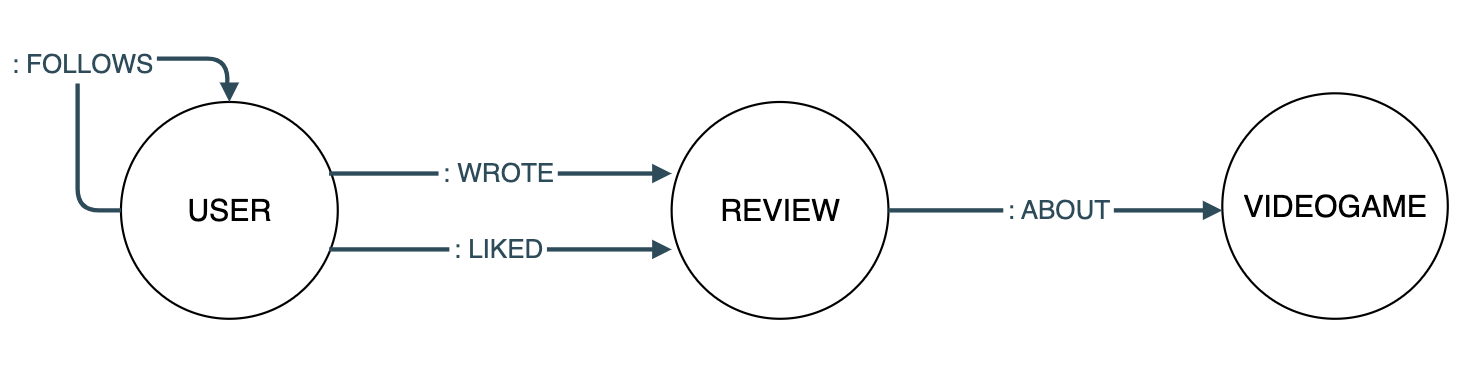
\includegraphics[width=1\textwidth]{chapter3/img/graph.png}
	\caption{Entities handled by \emph{GraphDB} and their relationships}
	\label{fig:graph}
\end{figure}
We handled the following entities via GraphDB (figure \ref{fig:graph}) :
\begin{itemize}
	\item User
	\item Videogame
	\item Review
\end{itemize}
At the very base of our project’s idea we find a social networking system. 
The graph database is exploited to keep track of the users within our network and mainly to manage and make the most out of their connections and relationships.
The graph database’s architecture we benefit from allow us to make efficient querying of relationships between users, to perform analytics and subsequent actions based on connection findings.
We decided to have a simplified representation of all the entities involved (users, reviews and videogames), that are stored in detail on a document database. Having the three entities over both the two different types of database we need to deal with consistency between MongoDB and Neo4j (we'll address this problem in the next section). 
The idea is to use this specific type of architecture to identify which users share the same taste in games, and then use this information to suggest new connections. 

The system will recommend two entities to a logged in user: users to follow and games to play. The first depends on the games that have being reviewed by the user, and the second depends on the users already followed. More details on the implementation will be provided later. 
\subsection{Nodes within the graph}
We have three types of nodes:
\begin{itemize}
    \item \emph{User} : simplified version of the MongoDB collection \emph{users} that for each user only keeps track of the \texttt{username}, that we remember has to be unique.
    \item \emph{Review} : simplified version of the MongoDB collection \emph{reviews}. For each review we have the \texttt{reviewID} (that uniquely identifies each review into the database) and the related \texttt{score}.
    \item \emph{Videogame} : simplified version of the MongoDB collection \emph{videogames}. We keep only the videogames' unique \texttt{name} attribute, that is enough for the queries we need to perform. 
\end{itemize}
we added these redundancies (all the information in Neo4j is a subset of the overall data stored in MongoDB) to have at our disposal solely the information needed to perform the queries we decided to implement using the strenghts of the graph database's architecture. 
\subsection{Relationships between nodes of the graph}
Here we look at the type of relationships within the graph:
\begin{itemize}
    \item \emph{Follows} : if the user \texttt{A} follows another user \texttt{B} there is a \texttt{:FOLLOWS} relationship from \texttt{A} to \texttt{B}
\begin{equation*}
\texttt{A} \xrightarrow{\texttt{:FOLLOWS}} \texttt{B}
\end{equation*}
    \item \emph{Wrote} : if the user \texttt{U} writes a review \texttt{R}, we create a \texttt{:WROTE} relationship from \texttt{U} to \texttt{R}
\begin{equation*}
\texttt{U} \xrightarrow{\texttt{:WROTE}} \texttt{R}
\end{equation*}
    \item \emph{Liked} : if the user \texttt{U} likes a review \texttt{R} we keep track of this by generating a \texttt{:LIKED} relationship from \texttt{U} to \texttt{R}
\begin{equation*}
\texttt{U} \xrightarrow{\texttt{:LIKED}} \texttt{R}
\end{equation*}
    \item \emph{About} : if a review \texttt{R} was written for the specific videogame \texttt{V} we need to create an \texttt{:ABOUT} relationship from \texttt{R} to \texttt{V} 
\begin{equation*}
\texttt{R} \xrightarrow{\texttt{:ABOUT}} \texttt{V}
\end{equation*}
\end{itemize}
\section{Distributed Database Design}
\subsection{Replicas}
\begin{figure}[hbt!]
	\centering
	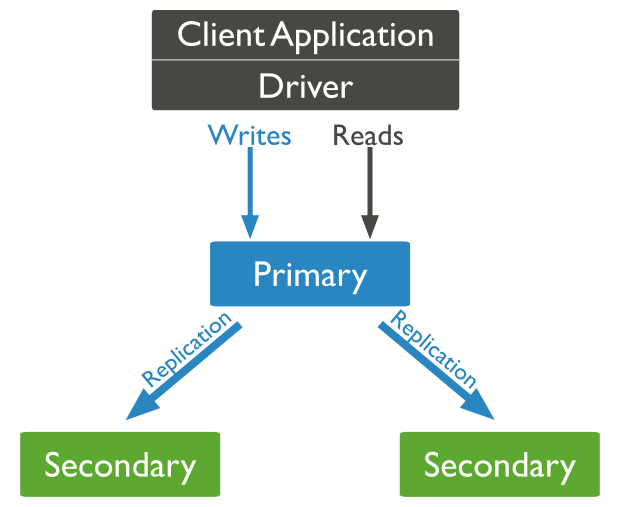
\includegraphics[width=0.5\textwidth]{chapter3/img/replica.png}
	\caption{Replica Set}
	\label{fig:replica}
\end{figure}
We were given the chance to exploit a cluster of three nodes for the project. We deployed one \emph{MongoDB replica} for each node (replicas were not implemented for \emph{Neo4j} since to do so we would have needed the \emph{Enterprise edition}). 
The \emph{primary} is the only member in the replica set that receives write operations (figure \ref{fig:replica}). MongoDB applies write operations on the primary and then records the operations on the primary's \emph{oplog}. \emph{Secondary} members replicate this log and apply the operations to their data sets.
All members of the replica set can accept read operations. By default, however, an application directs its read operations to the primary node.
\subsubsection{Consistency Level}
Consistency Level refers to the consistency between copies of data on different replicas. We consider data to be \emph{strictly consistent} if all replicas have the same data. Enforcing strong consistency, anyway, would be too costly and - even before that - unnecessary. Eventual consistency is sufficient : we'll have a \emph{write concern} (i.e. the level of acknowledgment requested from MongoDB for write operations on the \emph{Replica set}) with the \texttt{w} option set to 1, requesting acknowledgment that each write operation has been propagated to the primary in the replica set. Data can be rolled back if the primary steps down before the write operations have replicated to any of the secondaries (\texttt{w: 1} is specified into the \texttt{spring.data.mongodb.uri} placed in \texttt{application.properties}, under the \texttt{resources} directory of the project, where we also specify the \emph{read concern} \texttt{readConcernLevel=local}, i.e. \texttt{r: 1}). Early results of eventual consistency data queries might not have the most recent updates, it will take time for updates to reach replicas across the database cluster.
The consistency level has to be set according to several requirements. 
Returning the latest data for every query would result in high latency and delay, two aspects we need to be really careful about. We always need to keep in mind that we are working on a social networking system, in which engagement with the user has to be given the top one priority. By exploiting \emph{eventual consistency} results will be less consistent early on, but they will be provided much faster, with low latency. Facing inconsistency does not really represent a problem for the purposes of the application.


%\subsubsection{Write Concern}
%Write concern describes the level of acknowledgment requested from MongoDB for write operations to Replica sets
%(TO DO: relation with Async)
\subsection{Sharding}
Heavy loads on a server,  than in the specific case of our application may be due to a large number of users in our network, can be dealt with through a process of horizontal partitioning. Horizontal partitioning of a document database is often referred to as \emph{sharding} and it consists in dividing a database by documents into different sections (known as \emph{shards}) stored on separate servers. This process could be exploited to enable our document database to scale in order to meet a possibly growing demand for our application. Each server within the document database cluster will have only \emph{one} shard per server, so if our database is configured to replicate data, than a single shard will be stored on multiple servers. We'll consider sharding only for the Document side of our database, since the GraphDB architecture presents challenges for distributing the graph across multiple
servers: while a node can, of course, point to an adjacent node located on another machine, the overhead of routing the traversal across multiple machines eliminates the advantages of the graph database model, because inter-server communication is far more time consuming than local access. 

To implement sharding on the document side, we need to select a \emph{shard key} and a \emph{partitioning method}. The shard key specifies the values to use when grouping documents into different shards, so it is represented by one or more fields that need to exist in \emph{all} documents in a collection, and that should be chosen accordingly to the specific requests we expected to get from our clients, in order to optimize the response of the application. 
We can implement a hash-based sharding for Reviews and Comments, using their \emph{IDs} as sharding keys. In this perspective we would use hashing as a partitioning algorithm, which would be helpful to evenly balance the load on different servers by applying an hash function to the shard keys: with hash-based partitioning
new documents are distributed evenly across all members of the cluster.
Considering the possibility of having to deal with a larger and larger amount of \emph{Videogames}, on the other hand, we could shard the videogames' collection using as \emph{sharding key} the \texttt{release\_date} - an attribute that every \emph{videogame} has to have (which actually makes it exploitable to implement the \emph{key}). This particular type of sharding could significantly optimize some of the queries we often need to perform over the database. We can look specifically at the one implemented in order to return and show to the final users the \emph{newest} videogames, that was an operation specifically thought to advertise and keep the users updated on the latest releases, offering \emph{Company Managers} a showcase on which to advertise their new products. 
Whenever range partitioning is enabled and the shard key is continuously incremented, as it is in our case considering the \emph{release date}, we need to be careful, each time a new videogame is added to the database, to the fact that the load will tend to aggregate against only one of the shards, possibly unbalancing the cluster. However, we \emph{do not} consider the addition of new videogames to be so frequent that it could become critical, leading to problems.

%\emph{mongos} instances will pass the \emph{write concern} on to the shards
\subsection{Handling inter-databases consistency}
\begin{figure}[t]
	\centering
	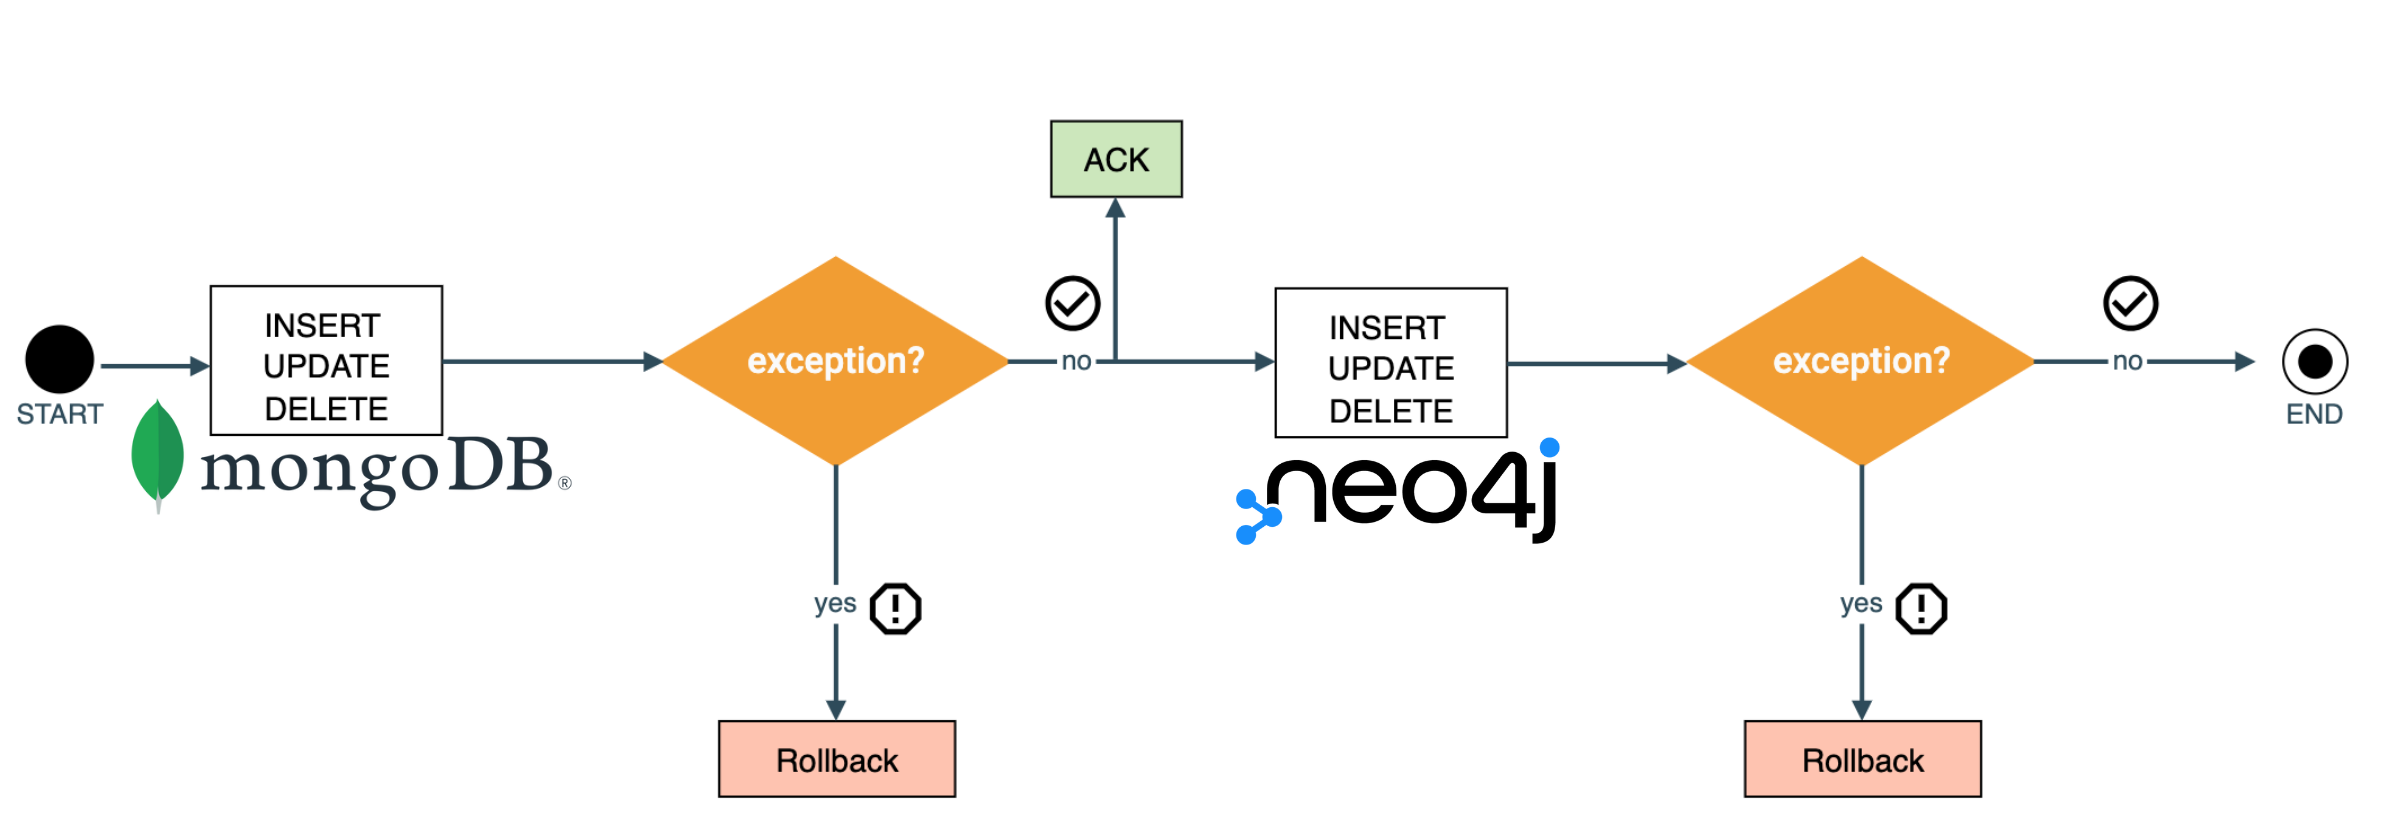
\includegraphics[width=1\textwidth]{chapter3/img/rollback.png}
	\caption{Handling consistency between \emph{MongoDB} and \emph{Neo4j}}
	\label{fig:rb}
\end{figure}
Having to deal with two different architectures (\emph{DocumentDB} and \emph{GraphDB}), we need to face the problem of redundancy and handle the consistency of data that are stored within both databases. 
Any rollback triggered by a failure of an insert, an update or a delete operation, can lead to inconsistencies. 
To address this problem, the system will start write operations on \emph{Neo4J} only when the same operation  is performed successfully on \emph{MongoDB}. Then, if any exception occurs when the updates over data on \emph{Neo4j} are attempted, then a rollback operation will be executed in order to bring back both the databases in a consistent state (just as shown in figure \ref{fig:rb}). All of this is made possible by the annotation \emph{@Transactional}, made available by Spring Data.
% NEW 
 
\subsubsection{High Availability, Eventual Consistency}
Eventual consistency is dealt with by exploiting the \emph{asynchronous execution support} in \emph{Spring} and the \emph{@Async} annotation.
The caller will not have to wait for the complete execution of the called method: annotating a method of a bean with \emph{@Async} will make it execute in a separate thread, thus increasing the availability of our application. 